\section{Evaluation}

We evaluate the adaptive tracing controller across five research questions. RQ1 asks whether the controller can determine when sufficient diagnostic evidence has been collected. RQ2 asks how accurate automatic tracing is compared with manual fixed-window profiling. RQ3 measures the overhead introduced by the controller. RQ4 compares the six short-burst stopping policies. RQ5 identifies which runtime signals are most useful for deciding when to stop heavy GPU tracing.


% \subsection{Experimental Setup}

% Experiments run on two single-GPU cloud platforms: an NVIDIA L4 (24\,GB, Ada Lovelace, \texttt{sm\_89}) as the primary platform for all research questions, and an NVIDIA A100 (40\,GB, Ampere, \texttt{sm\_80}) for cross-GPU validation in RQ1. All vLLM scenarios serve \texttt{Qwen/Qwen2.5-7B-Instruct} using vLLM v0.10.2 in BFloat16 precision. Controller and policy parameters are fixed across experiments as listed in Table~\ref{tab:setup-params}. Each workload uses five repetitions for microbenchmarks or three seeded repetitions for vLLM experiments, with results reported as means.

\subsection{Experimental Setup}

Experiments run on two single-GPU cloud platforms: an NVIDIA L4 (24,GB, Ada Lovelace, \texttt{sm\_89}) as the primary platform for all research questions, and an NVIDIA A100 (40,GB, Ampere, \texttt{sm\_80}) for cross-GPU validation in RQ1. All vLLM scenarios use vLLM v0.10.2~\cite{kwon2023vllm}, an open-source inference engine that implements PagedAttention for efficient KV-cache management and exposes an OpenAI-compatible HTTP API. The system serves \texttt{Qwen/Qwen2.5-7B-Instruct}~\cite{qwen2025}, a 7-billion-parameter instruction-tuned model, in BFloat16 precision.

Unless otherwise stated, vLLM uses its default configuration and automatically allocates the KV cache from available GPU memory. This provides approximately 64,704 KV-cache tokens on the 24,GB L4 host and 334,016 tokens on the 40,GB A100 host. CUDA graph capture remains enabled throughout the experiments. Although graph replay groups multiple kernel launches into a single CPU-side submission, Nsight Systems still records the individual GPU kernels within each replayed graph; consequently, T2 kernel-level evidence, including execution time, launch frequency, and duration distributions, is unaffected.

Controller and policy parameters are fixed across experiments as listed in Table~\ref{tab:setup-params}. Each workload uses five repetitions for microbenchmarks or three seeded repetitions for vLLM experiments, with results reported as means.

\subsubsection{Controller Parameters}

Table~\ref{tab:setup-params} lists the controller and policy parameters held constant across all experiments.

\begin{table}[h]
\centering
\caption{Controller and policy parameters used in all experiments.}
\label{tab:setup-params}
\footnotesize
\setlength{\tabcolsep}{4pt}
\begin{tabularx}{\columnwidth}{@{}l l >{\raggedright\arraybackslash}X@{}}
\toprule
\textbf{Parameter} & \textbf{Value} & \textbf{Notes} \\
\midrule
Evidence window size               & 10\,s              & All experiments \\
Automatic burst duration           & $\approx$10--12\,s & Bounded by target process duration \\
Fixed-window burst duration        & $\approx$17--24\,s & $1.6\times$--$2.0\times$ automatic \\
Stability window count $K$         & 2                  & \textsc{SS}, \textsc{HS} \\
Repeated burst count $N$           & 3                  & \textsc{RFB} \\
Maximum tracing budget             & 6 bursts/episode   & All policies \\
Latency recovery ratio             & 1.10               & \textsc{CR}, \textsc{HS} \\
GPU utilization recovery threshold & 60\%               & \textsc{CR}, \textsc{HS} \\
NVML polling interval              & 0.5\,s             & T1 collection \\
\bottomrule
\end{tabularx}
\end{table}


\subsubsection{Repetitions and Seeds}

Microbenchmark experiments use five independent repetitions per workload, while vLLM serving experiments use three seeded repetitions per scenario; all results report means across repetitions and, where relevant, 95\% confidence interval half-widths.



\subsection{RQ1: Can the Controller Determine When Sufficient Diagnostic Evidence Has Been Collected?}

\subsubsection{Metrics}

We evaluate evidence sufficiency using trace-time saved, expected-label match rate, and burst-count stability, measured as the standard deviation ($\sigma$) of profiler bursts across repetitions. Trace-time saved is the reduction in total profiler-active duration relative to the fixed-window baseline. An RQ1 result is considered successful when trace-time savings are at least 25%, the expected-label match rate is at least 0.95, and $\sigma \leq 0.25$.

\subsubsection{Microbenchmark Results}

Table~\ref{tab:rq1-micro} reports the RQ1 microbenchmark results for both the L4 and A100 platforms across five repetitions per workload.

\begin{table}[h]
\centering
\caption{RQ1 microbenchmark results: automatic vs.\ fixed-window profiler duration (mean over 5 repetitions). All rows pass the combined success criterion.}
\label{tab:rq1-micro}
\resizebox{\columnwidth}{!}{%
\begin{tabular}{llrrrrr}
\toprule
\textbf{GPU} & \textbf{Workload} & \textbf{Auto (s)} & \textbf{Fixed (s)} &
\textbf{Saved (\%)} & \textbf{Match rate} & \textbf{Burst $\sigma$} \\
\midrule
A100 & \texttt{compute\_bound}   & 10.4 & 16.7 & 37.6 & 1.0 & 0.0 \\
A100 & \texttt{launch\_overhead} & 11.9 & 23.2 & 48.5 & 1.0 & 0.0 \\
A100 & \texttt{mixed}            & 10.2 & 16.8 & 39.2 & 1.0 & 0.0 \\
\midrule
L4   & \texttt{compute\_bound}   & 12.4 & 18.1 & 31.6 & 1.0 & 0.0 \\
L4   & \texttt{launch\_overhead} & 13.0 & 24.0 & 45.8 & 1.0 & 0.0 \\
L4   & \texttt{mixed}            & 12.0 & 18.5 & 35.4 & 1.0 & 0.0 \\
\bottomrule
\end{tabular}%
}
\end{table}

The controller saves between 31.6\% and 48.5\% of profiler duration across all six workload-platform combinations while maintaining a perfect expected-label match rate of 1.0. Burst count standard deviation is 0.0 in every case: per-repetition logs show exactly one profiler burst in all 30 repetitions. This reflects the microbenchmark design, not insufficient variation between repetitions: each workload presents a single, unambiguous bottleneck signature from the first suspicious window, so diagnosis stability is already satisfied after one burst regardless of timing jitter. This single-burst convergence is specific to the controlled microbenchmarks; RQ2 and RQ4 (Section~\ref{sec:rq4}) show burst counts greater than one when the bottleneck class is less immediately separable. All rows pass the combined RQ1 success criterion.

Savings are consistently higher for \texttt{launch\_overhead\_or\_small\_kernel} than for \texttt{compute\_bound} or \texttt{mixed} on both GPUs. This is expected: the kernel summary for a high-launch-rate workload reveals its bottleneck class (many short kernels) after a short burst, allowing the stability condition to be satisfied quickly, whereas compute-bound and mixed workloads require a slightly longer burst to produce a stable GEMM-dominated summary.

Per-condition savings are stable: 95\% CI half-widths range from $\pm 0.5$ to $\pm 2.7$ points across the six combinations, an order of magnitude smaller than the 17-point spread between conditions.

% The A100 results are consistent in direction with the L4 results, with savings ranging from 37.6\% to 48.5\% on the A100 versus 31.6\% to 45.8\% on the L4. The modest difference in absolute savings is attributable to the A100's higher memory bandwidth and faster kernel execution times, which allow the diagnosis stability condition to be reached sooner within a burst.


\subsubsection{vLLM Serving Results}

On the \texttt{queue\_pressure} vLLM serving scenario, across three seeded repetitions on the L4, the controller reduces mean profiler duration from 133.5\,s (fixed-window) to 104.6\,s (automatic) -- a 21.7\% reduction (95\% CI $\pm 4.0$pp) -- while maintaining 100\% request success in every repetition.

\subsubsection{RQ1: Answer}

Yes. The adaptive controller determines when sufficient diagnostic evidence has been collected and stops heavy GPU tracing 21.7\%--48.5\% earlier than a manual fixed-window baseline across all evaluated workloads and GPU platforms, without sacrificing diagnosis accuracy.
\subsection{RQ2: How Accurate Is Automatic GPU Tracing Compared with Manual Profiling?}

\subsubsection{Metrics}

We evaluate diagnosis accuracy using expected-label match rate, ambiguous or unknown rate, time-to-diagnosis, and automatic-versus-fixed-window disagreement rate. Expected-label match rate is evaluated separately for automatic and fixed-window modes, with a success threshold of at least 0.95; the ambiguous or unknown rate has a target of at most 0.05. Time-to-diagnosis is the mean elapsed time from run start to the first window assigned the expected label. Disagreement measures the fraction of paired windows for which automatic and fixed-window modes assign different labels; disagreement alone is not an accuracy failure when both modes match the expected label in their respective suspicious windows.

\subsubsection{Microbenchmark Results}

Across all three L4 microbenchmark workloads and five repetitions each, automatic and fixed-window tracing achieved a 1.0 expected-label match rate and a 0.0 ambiguous rate. Both modes identified the expected bottleneck in the first evidence window, within approximately 5--6\,s.

\subsubsection{vLLM Multiclass Results}

Table~\ref{tab:rq2-vllm} reports RQ2 accuracy for the vLLM multiclass long-run experiments (three seeded repetitions per scenario, 402 per-window records total across six scenarios).

\begin{table*}[t]
\centering
\caption{RQ2 vLLM multiclass accuracy (3 seeds per scenario, L4). All six scenarios pass
all accuracy criteria in both modes. Auto trace and fixed-window trace columns report total
profiler duration across all repetitions.}
\label{tab:rq2-vllm}
\footnotesize
\setlength{\tabcolsep}{4pt}
\renewcommand{\arraystretch}{0.95}
\begin{tabular}{llrrrrrr}
\toprule
\textbf{Scenario} & \textbf{Mode} & \textbf{Match} & \textbf{Ambig.} &
\textbf{TTD (s)} & \textbf{Disagree} & \textbf{Trace (s)} & \textbf{Kernels} \\
\midrule
\texttt{healthy}
  & Auto  & 1.0 & 0.0 & 10.0 & \multirow{2}{*}{0.00} & 301.3 & 730K \\
  & Fixed & 1.0 & 0.0 & 10.0 &                        & 391.9 & 1380K \\
\midrule
\texttt{queue\_pressure}
  & Auto  & 1.0 & 0.0 & 10.0 & \multirow{2}{*}{0.00} & 309.7 & 748K \\
  & Fixed & 1.0 & 0.0 & 10.0 &                        & 403.4 & 1380K \\
\midrule
\texttt{long\_prompt}
  & Auto  & 1.0 & 0.0 & 10.0 & \multirow{2}{*}{0.25} & 290.4 & 732K \\
  & Fixed & 1.0 & 0.0 & 10.0 &                        & 381.0 & 1380K \\
\midrule
\texttt{long\_output}
  & Auto  & 1.0 & 0.0 & 10.0 & \multirow{2}{*}{0.00} & 291.0 & 729K \\
  & Fixed & 1.0 & 0.0 & 10.0 &                        & 397.1 & 1380K \\
\midrule
\texttt{compute\_saturation}
  & Auto  & 1.0 & 0.0 & 10.0 & \multirow{2}{*}{0.00} & 336.8 & 757K \\
  & Fixed & 1.0 & 0.0 & 10.0 &                        & 415.1 & 1380K \\
\midrule
\texttt{kv\_cache\_pressure}
  & Auto  & 1.0 & 0.0 & 10.0 & \multirow{2}{*}{0.00} & 329.4 & 731K \\
  & Fixed & 1.0 & 0.0 & 10.0 &                        & 449.3 & 1380K \\
\bottomrule
\end{tabular}
\end{table*}

% All six vLLM serving scenarios pass all accuracy criteria in both automatic and fixed-window modes. The expected-label match rate is 1.0, the ambiguous rate is 0.0, and time-to-diagnosis is the first 10\,s evidence window for every scenario and mode.
Automatic and fixed-window tracing satisfy all accuracy criteria across the six vLLM serving scenarios (Table~\ref{tab:rq2-vllm}), with a perfect expected-label match rate, zero ambiguous rate, and diagnosis in the first 10\,s evidence window.

% The disagreement rate is 0.0 for five of the six scenarios. The non-zero disagreement for \texttt{long\_prompt} (0.25) is again a sequence-level difference rather than an accuracy failure: both modes match the expected label on their respective suspicious windows.
Non-zero disagreement rates reflect sequence-level differences rather than diagnosis failures. \texttt{long\_prompt} is the only vLLM scenario with non-zero disagreement (0.25), because automatic mode stops collecting bursts earlier, so automatic and fixed-window tracing do not always assign profiler-enriched labels to the same windows; both modes still assign the correct expected label on every suspicious window.


% Across all six vLLM scenarios, automatic mode uses 1,858\,s of total profiler time against 2,438\,s for fixed-window mode, capturing 1,460K kernel instances against 2,759K for fixed-window mode. Automatic mode achieves the same accuracy while profiling for 23.8\% less time and recording 47.1\% fewer kernel instances.

Across all six vLLM scenarios, automatic mode achieves the same diagnosis accuracy as fixed-window tracing while profiling for 23.8\% less time and recording 47.1\% fewer kernel instances.


\subsubsection{RQ2: Answer}

Automatic GPU tracing matches the diagnosis accuracy of manual fixed-window profiling exactly: an expected-label match rate of 1.0 and an ambiguous rate of 0.0 across all microbenchmark workloads and all six vLLM serving scenarios, with time-to-diagnosis at the first evidence window in every case. Automatic mode reaches this accuracy using 23.8\% less profiler time and recording 47.1\% fewer kernel instances.

\subsection{RQ3: Does Automatic GPU Tracing Introduce Overhead Compared with Manual Profiling?}

We study overhead from two complementary angles. The first is \emph{profiler-cost overhead}: how much profiler time and how many profiled kernel instances does automatic tracing use compared with fixed-window profiling? The second is \emph{runtime perturbation}: does running the cheap controller metrics alongside vLLM introduce measurable degradation in request latency or throughput?

\subsubsection{Metrics}

\begin{itemize}
  \item \textbf{Trace-time saved (\%) and kernel instances avoided (\%).}
    Reduction in profiler-active duration and in the number of kernel instances recorded by the profiler, relative to the fixed-window baseline.
  \item \textbf{p95 latency regression (\%).}
    Change in p95 request latency between cheap-metrics mode and no-profiler mode, computed as $(p95_{\text{cheap}} - p95_{\text{none}}) / p95_{\text{none}} \times 100$. Positive values indicate regression; negative values indicate improvement.
  \item \textbf{Throughput change (\%).}
    Change in requests per second between cheap-metrics mode and no-profiler mode.
  \item \textbf{Request success rate.}
    Fraction of requests that completed successfully. Must remain at 100\%.
\end{itemize}

The RQ3 success criteria are: positive trace-time savings, positive kernel-instance reduction, p95 latency regression $\leq 5\%$, and request success rate of 100\%.

\subsubsection{Profiler-Cost Overhead}

Combining the RQ1 and RQ2 artifacts (Tables~\ref{tab:rq1-micro}--\ref{tab:rq2-vllm}), automatic tracing reduces profiler duration by 18.9\%--48.5\% and captured kernel instances by 42.9\%--78.2\% across all workloads, relative to the fixed-window baseline and while preserving a diagnosis match rate of 1.0. Microbenchmark workloads show higher savings than vLLM scenarios because their bottleneck classes stabilize more quickly.

\subsubsection{Dedicated Runtime Perturbation}

To isolate the cost of the cheap controller metrics, we compare a \emph{no-profiler} baseline against a \emph{cheap-metrics-only} mode (NVML polling and windowed metric aggregation, no Nsight profiling), randomizing which mode runs first in each repetition to control for run-order effects, across five randomized repetitions of \texttt{queue\_pressure} and three of \texttt{healthy}. All rows pass the RQ3 criteria.

The cheap controller metrics introduce no measurable p95 latency regression on either scenario. For \texttt{queue\_pressure} the mean p95 latency is 3.6\% \emph{lower} in cheap-metrics mode (5 reps, 95\% CI $\pm 6.3$ points), and for \texttt{healthy} the regression is $+0.6\%$ (3 reps, 95\% CI $\pm 1.9$ points), well within the 5\% threshold. Both intervals are wide given the small repetition counts, but even \texttt{queue\_pressure}'s upper bound ($+2.7\%$) clears the threshold with margin. Request success remains at 100\% in both scenarios and both modes.

Throughput change is small ($-0.5\%$ to $-1.0\%$) but more sensitive to run order than p95 latency; we report it as context rather than as a hard criterion.

\subsubsection{RQ3: Answer}

Automatic tracing reduces profiler cost substantially relative to fixed-window profiling without degrading serving performance: profiler duration drops by 18.9\%--48.5\% and captured kernel instances by 42.9\%--78.2\%. The cheap controller metrics introduce less than 1\% mean p95 latency change in the serving workload in five randomized repetitions, confirming that the controller overhead is negligible.


\subsection{RQ4: Which Short-Burst GPU Tracing Policies Work Best?}
\label{sec:rq4}

\subsubsection{Evaluation Approach}

RQ4 compares the six stopping policies via offline replay over real L4 vLLM window evidence, avoiding additional expensive Nsight executions per policy. Each policy is replayed over the same per-window evidence streams, so differences in outcome are attributable solely to the stopping condition rather than to workload variation or profiler noise. This assumes a policy's stopping choice does not meaningfully change later windows' evidence; we expect this confound to be small since T0/T1 collection is always-on and policy-independent, and RQ3 bounds the profiler's own T0/T1 perturbation at under 1\%.

We use two replay datasets. The \emph{stable replay} uses the real automatic-mode windows from the six vLLM serving scenarios across three seeds (18 streams). In this dataset the correct bottleneck label appears in the first suspicious window for every stream, making it an easy diagnostic setting. The \emph{ambiguity stress replay} uses the same 18 streams with the first suspicious window in each stream relabeled as unknown, modeling the realistic case where a single burst is insufficient. The stress dataset is the primary discriminating evaluation because it separates policies that can handle ambiguous early windows from those
that cannot.

\subsubsection{Metrics}

We report mean top-1 accuracy, premature-stop rate, re-escalation-needed rate (the fraction of streams with suspicious windows remaining after the policy stops), mean heavy-trace duration, and duration saved relative to the Repeated Fixed Burst baseline ($N=3$). These are combined into a composite score weighted 40\% accuracy, 25\% premature-stop avoidance, 20\% re-escalation avoidance, and 15\% cost-efficiency.\footnote{Composite score $= 0.40 \times \text{accuracy} + 0.25 \times (1 - \text{premature-stop rate}) + 0.20 \times (1 - \text{re-escalation rate}) + 0.15 \times \text{cost-efficiency}$, where cost-efficiency is the normalised inverse of mean trace duration.}

\subsubsection{Stable Replay Results}

The stable replay is not the discriminating condition --- every policy reaches top-1 accuracy of 1.0 with zero premature stops --- so its results are summarized in text rather than a table. \textsc{CR} and \textsc{HS} avoided re-escalation entirely but required 34.9\,s of tracing per episode, whereas \textsc{FB} used 10.0\,s but left suspicious windows after stopping. \textsc{MU} and \textsc{SS} were Pareto-dominated by \textsc{FB}: they incurred twice the tracing cost (20.0\,s) without improving accuracy or re-escalation rate. \textsc{RFB} fell between these extremes (30.0\,s, re-escalation rate 0.8) and remained Pareto-efficient only because no other policy matched its particular cost--reliability point.

\subsubsection{Ambiguity Stress Replay Results}

Table~\ref{tab:rq4-stress} reports policy rankings on the ambiguity stress dataset, which
is the primary discriminating evaluation.

\begin{table*}[t]
\centering
\caption{RQ4 ambiguity stress policy ranking (18 streams, first window relabeled as
unknown). \textsc{FB} fails entirely; multi-window policies recover to top-1 accuracy
of 1.0.}
\label{tab:rq4-stress}
\footnotesize
\setlength{\tabcolsep}{4pt}
\renewcommand{\arraystretch}{0.95}
\begin{tabular}{clrrrrrrl}
\toprule
\textbf{Rank} & \textbf{Policy} & \textbf{Top-1} & \textbf{Premature} &
\textbf{Re-esc.} & \textbf{Trace (s)} & \textbf{Saved (\%)} &
\textbf{Score} & \textbf{Pareto} \\
\midrule
1 & \textsc{CR} & 1.0 & 0.0 & 0.0 & 34.9 & $-16.3$ & 0.868 & yes \\
2 & \textsc{HS} & 1.0 & 0.0 & 0.0 & 34.9 & $-16.3$ & 0.868 & yes \\
3 & \textsc{MU} & 1.0 & 0.0 & 0.8 & 30.0 &    0.0  & 0.720 & yes \\
4 & \textsc{RFB} & 1.0 & 0.0 & 0.8 & 30.0 &   0.0  & 0.720 & yes \\
5 & \textsc{SS} & 1.0 & 0.0 & 0.8 & 30.0 &    0.0  & 0.720 & yes \\
6 & \textsc{FB} & 0.0 & 1.0 & 1.0 & 10.0 & $+66.7$ & 0.112 & yes \\
\bottomrule
\end{tabular}
\end{table*}

The stress dataset clearly separates one-burst and multi-burst policies.
\textsc{FB} fails completely: its top-1 accuracy drops to 0.0 and its premature-stop rate
rises to 1.0, because it commits to the ambiguous first-window unknown label and never
collects the additional burst needed to reach the concrete diagnosis.
Despite this failure, \textsc{FB} still shows Pareto-efficient in Table~\ref{tab:rq4-stress}, since no policy beats it on cost alone; Pareto status must therefore be read alongside accuracy and premature-stop rate, not as a standalone selection criterion.

All five multi-window policies recover to a top-1 accuracy of 1.0 and a premature-stop
rate of 0.0.
\textsc{CR} and \textsc{HS} again rank highest with a re-escalation rate of 0.0,
confirming their robustness as safety-first policies: they wait for both diagnosis
stability and workload recovery before stopping, ensuring no suspicious windows remain.

\textsc{MU}, \textsc{SS}, and \textsc{RFB} are tied at rank 3--5 with a re-escalation
rate of 0.83 and a mean trace duration of 30\,s. \textsc{MU} and \textsc{SS} are
preferable to \textsc{RFB} since they stop on evidence convergence rather than a
fixed burst count.

\subsubsection{Policy Tradeoff Analysis}

Figure~\ref{fig:rq4-tradeoff} illustrates the cost--safety tradeoff across the six
policies on the stress dataset.

\begin{figure}[t]
\centering
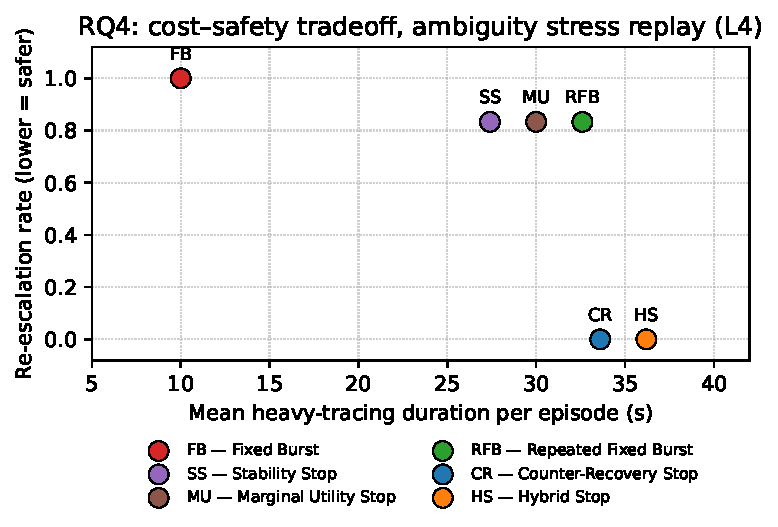
\includegraphics[width=\columnwidth]{figures/rq4_tradeoff.pdf}
\caption{Cost--safety tradeoff across the six stopping policies on the ambiguity stress dataset (Table~\ref{tab:rq4-stress}). \textsc{CR} and \textsc{HS} achieve zero re-escalation at higher trace cost; \textsc{MU}, \textsc{RFB}, and \textsc{SS} trade a 0.8 re-escalation rate for lower cost; \textsc{FB} is cheapest but fails outright (top-1 accuracy 0.0) rather than merely re-escalating.}
\label{fig:rq4-tradeoff}
\end{figure}

\subsubsection{RQ4: Answer}

No single policy dominates all dimensions, so the right choice depends on operator priorities. For safety-first deployments, \textsc{Hybrid Stop} and \textsc{Counter-Recovery Stop} eliminate re-escalation entirely and are robust to ambiguous first windows, at the cost of about 16\% more trace budget than \textsc{RFB}. For budget-aware deployments, \textsc{Stability Stop} and \textsc{Marginal Utility Stop} achieve 1.0 top-1 accuracy with 33\% less trace time than the recovery-gated policies, accepting a re-escalation rate of approximately 0.83. \textsc{Fixed Burst} is not robust as a standalone policy: it fails completely when the first profiler window is ambiguous, with a top-1 accuracy of 0.0 and a premature-stop rate of 1.0 on the stress dataset.
\subsection{RQ5: Which Runtime Signals Are Most Useful for Deciding When to Stop Heavy GPU Tracing?}
\label{sec:rq5}

\subsubsection{Evaluation Approach}

RQ5 evaluates the nine candidate stopping signals defined in Section~\ref{sec:stopping-policies} on two datasets.

\begin{itemize}
  \item[] \textbf{Real enriched L4 runs.} 18 vLLM serving runs (6 scenarios $\times$ 3 seeds, 60\,s per run) collected with the enriched window schema that includes non-sparse baseline ratio fields, recovery streak counters, and diagnosis confidence and margin fields. These runs provide a realistic serving signal distribution for evaluating which signals identify correct stopping points.
  \item[] \textbf{Ambiguity stress replay.} The same stress dataset used in RQ4 (first suspicious window relabeled as unknown). This dataset tests whether a signal fires on ambiguous stopping points as well as correct ones; a signal that cannot distinguish between the two is not safe to use as a standalone stopping criterion.
\end{itemize}

A signal is considered \emph{paper-ready} if it satisfies all three of the following criteria simultaneously: (1) precision $\geq 0.90$ on both datasets, (2) correct-stop F1 $\geq 0.70$ on the stress replay, and (3) ambiguous-stop F1 $\leq 0.10$ on the stress replay. Criterion (3) is the strictest filter: a signal that fires reliably on correct windows but also fires on ambiguous windows would cause the controller to stop too early when the diagnosis has not yet converged.

\subsubsection{Signal Ranking Results}

Table~\ref{tab:rq5-signals} reports precision, recall, and F1 for each candidate signal across the two evaluation datasets, together with the paper-ready verdict.

\begin{table*}[t]
\centering
\caption{RQ5 stopping signal ranking. Signals are sorted by composite score. Only
\texttt{diagnosis\_stable\_2} passes all paper-ready criteria.}
\label{tab:rq5-signals}
\footnotesize
\setlength{\tabcolsep}{4pt}
\renewcommand{\arraystretch}{0.95}
\begin{tabular}{lrrrrrrl}
\toprule
& \multicolumn{3}{c}{\textbf{Real enriched}} &
  \multicolumn{3}{c}{\textbf{Stress replay}} & \\
\cmidrule(lr){2-4} \cmidrule(lr){5-7}
\textbf{Signal} & \textbf{Prec.} & \textbf{Rec.} & \textbf{F1} &
\textbf{Prec.} & \textbf{F1 (correct)} & \textbf{F1 (ambig.)} &
\textbf{Paper-ready} \\
\midrule
\texttt{diagnosis\_stable\_2}   & 1.000 & 0.860 & 0.925 & 1.000 & 0.786 & 0.000 & \textbf{yes} \\
\texttt{latency\_recovered}     & 1.000 & 1.000 & 1.000 & 0.739 & 0.850 & 0.414 & no \\
\texttt{throughput\_recovered}  & 1.000 & 0.884 & 0.938 & 0.778 & 0.800 & 0.333 & no \\
\texttt{queue\_delay\_recovered}& 1.000 & 0.659 & 0.794 & 0.739 & 0.850 & 0.414 & no \\
\texttt{diagnosis\_margin\_clear}& 1.000 & 0.744 & 0.853 & 0.000 & 0.000 & 0.000 & no \\
\texttt{diagnosis\_changed}     & 1.000 & 0.465 & 0.635 & 1.000 & 0.522 & 0.000 & no \\
\texttt{gpu\_util\_recovered}   & 0.000 & 0.000 & 0.000 & 0.000 & 0.000 & 0.000 & no \\
\texttt{memory\_pressure\_low}  & 0.000 & 0.000 & 0.000 & 0.000 & 0.000 & 0.000 & no \\
\texttt{kernel\_duration\_stable}& 0.000 & 0.000 & 0.000 & 0.000 & 0.000 & 0.000 & no \\
\bottomrule
\end{tabular}
\end{table*}

\texttt{diagnosis\_stable\_2} is the only signal passing all three paper-ready criteria (Table~\ref{tab:rq5-signals}).

\subsubsection{Analysis of Individual Signal Groups}

\paragraph{Diagnosis-evidence signals.}
\texttt{diagnosis\_stable\_2} is the strongest and most defensible signal because it is derived directly from the kernel-level evidence the controller has already collected. It requires no external baseline calibration and does not depend on the workload's utilization or request rate returning to a specific threshold. Its main limitation is recall: on the real enriched runs it fires on 86\% of correct stopping points rather than all of them, meaning it occasionally requires one additional window before triggering.
\texttt{diagnosis\_margin\_clear} is promising on the real enriched runs (F1 0.853) but scores 0.000 on the stress replay, because the stress dataset predates the enriched schema and the margin field is absent.

\texttt{diagnosis\_changed} has perfect precision but low recall (F1 0.635 on real enriched runs). It is better understood as a \emph{continuation signal} than a stopping signal: when the diagnosis changes from one window to the next, the controller should continue tracing rather than stop. This is the inverse of its intended stopping role.

\paragraph{Recovery signals.}
\texttt{latency\_recovered} and \texttt{queue\_delay\_recovered} achieve the highest F1scores on the real enriched runs (1.000 and 0.794 respectively) but fail the paper-ready ambiguous-stop criterion with stress replay F1 values of 0.414. These signals fire on ambiguous stress windows because the stress transformation only relabels the diagnosis field, not the request latency values---latency recovery can therefore be observed even when the diagnosis is still unknown. They are valuable as supporting signals within the \textsc{CR} and \textsc{HS} policies, but they are not safe as standalone stopping signals.

\texttt{throughput\_recovered} shows a similar pattern: high F1 on real enriched runs (0.938) but fails the ambiguity criterion (stress F1 0.333).

\paragraph{GPU counter signals.}
At default thresholds (60\% util, 95\% memory), both score 0.000 since utilization never drops that low (observed range: 92.4--99.4\% util, 96.7--97.7\% memory). Recalibrating util to 99\% raises \texttt{gpu\_util\_recovered}'s recall to 0.953, but it then fires on 100\% of ambiguous windows (F1 0.419), violating the safety criterion; \texttt{memory\_pressure\_low} stays near-uninformative (recall 0.054) even at 97.5\%.

\paragraph{Kernel duration stability.}
\texttt{kernel\_duration\_stable} scores 0.000 because it requires two successive T2 bursts, and the \textsc{FB} policy used as the comparison baseline never collects a second burst.

\subsubsection{RQ5: Answer}

Diagnosis stability is the only stopping signal that is simultaneously precise, informative, and safe against ambiguous early windows. \texttt{diagnosis\_stable\_2} is the sole signal that passes all paper-ready criteria: it achieves 1.000 precision and an F1 of 0.925 on real enriched L4 runs, and never fires on ambiguous stopping points (stress ambiguous-stop F1 of 0.000). Recovery signals (\texttt{latency\_recovered}, \texttt{throughput\_recovered}) are strong on non-ambiguous workloads but fail the ambiguity safety criterion, making them suitable as supporting signals within \textsc{HS} and \textsc{CR} but not as standalone stopping criteria. GPU counter signals (\texttt{gpu\_util\_recovered}, \texttt{memory\_pressure\_low}) are inoperative for saturated LLM inference workloads.

